\begin{center}
    \begin{large}
    Cp 3 - Condicionales\\
    Curso \academicyear\\
    \end{large}
    \begin{figure}[h]
    	\centering
    	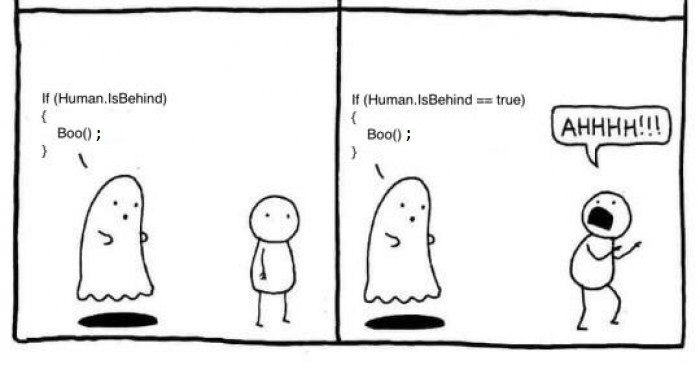
\includegraphics[width=0.6\linewidth]{cp3/conditional.jpg}
    \end{figure}
\end{center}

\section{Divisible}
Implemente un programa que reciba dos enteros y determine si el primero es divisible por el segundo.
\subsection*{Ejemplos:}
\begin{itemize}
    \item Entrada: \texttt{10, 2}\\
          Salida: \texttt{10 es divisible por 2.}
    \item Entrada: \texttt{15, 4}\\
          Salida: \texttt{15 no es divisible por 4.}
    \item Entrada: \texttt{20, 5}\\
          Salida: \texttt{20 es divisible por 5.}
    \item Entrada: \texttt{7, 3}\\
          Salida: \texttt{7 no es divisible por 3.}
\end{itemize}


\ifshowanswers
\section*{Respuesta:}
\begin{lstlisting}
Console.WriteLine("Introduce el dividendo:");
int a = int.Parse(Console.ReadLine() ?? string.Empty);
Console.WriteLine("Introduce el divisor:");
int b = int.Parse(Console.ReadLine() ?? string.Empty);

if (b != 0 && a % b == 0)
{
    Console.WriteLine($"{a} es divisible por {b}");
}
else
{
    Console.WriteLine($"{a} no es divisible por {b}");
}
\end{lstlisting}
\fi

\section{Mayor}
Implemente un programa que lea tres enteros de la consola e imprima el mayor.
\subsection*{Ejemplos:}
\begin{itemize}
    \item Entrada: \texttt{3, 5, 2}\\
          Salida: \texttt{El mayor número es 5.}
    \item Entrada: \texttt{10, 7, 10}\\
          Salida: \texttt{El mayor número es 10.}
    \item Entrada: \texttt{-1, -5, -3}\\
          Salida: \texttt{El mayor número es -1.}
    \item Entrada: \texttt{8, 8, 8}\\
          Salida: \texttt{El mayor número es 8.}
\end{itemize}

\section{Calculadora}
Implemente un programa que lea de la consola dos enteros y un operador (+, -, /, *) y realice la operación correspondiente entre ellos e imprima el resultado en consola.
\begin{itemize}
    \item Entrada: \texttt{5, 3, +}\\
    Salida: \texttt{El resultado de 5 + 3 es: 8}
    
    \item Entrada: \texttt{10, 4, -}\\
    Salida: \texttt{El resultado de 10 - 4 es: 6}
    
    \item Entrada: \texttt{8, 7, *}\\
    Salida: \texttt{El resultado de 8 * 7 es: 56}
    
    \item Entrada: \texttt{9, 3, /}\\
    Salida: \texttt{El resultado de 9 / 3 es: 3}
    
    \item Entrada: \texttt{5, 0, /}\\
    Salida: \texttt{Error: División por cero.}
\end{itemize}

\section{Carnet, de nuevo}
Implemente un programa que le pida al usuario su número de identidad y determine su sexo. El sexo puede determinarse por el penúltimo dígito del número de identidad (par masculino, impar femenino).

\subsection*{Ejemplos}
\begin{itemize}
    \item Entrada: \texttt{02020966175}\\
          Salida: \texttt{Femenino}
    
    \item Entrada: \texttt{04102566345}\\
          Salida: \texttt{Masculino}
    
    \item Entrada: \texttt{05031278457}\\
          Salida: \texttt{Femenino}
\end{itemize}



\ifshowanswers
\section*{Respuesta:}
\begin{lstlisting}
Console.WriteLine("Ingrese su número de identidad:");
long idNumber = long.Parse(Console.ReadLine() ?? string.Empty);
long penultimateDigit = idNumber / 10 % 10;
Console.WriteLine(penultimateDigit % 2 == 0 ? "Masculino" : "Femenino");
\end{lstlisting}
\fi

\section{Valor absoluto}
Implemente un programa que reciba un número entero \( x \) de la consola y calcule su valor absoluto. El valor absoluto de un número \( x \) se define como el número sin su signo, es decir, la distancia de \( x \) al origen en la recta numérica. No utilice Math.Abs.

La función del valor absoluto \( |x| \) se define de la siguiente manera:
\[
|x| =
\begin{cases} 
x & \text{si } x \geq 0 \\
-x & \text{si } x < 0
\end{cases}
\]

\subsection*{Ejemplos}
\begin{itemize}
    \item Entrada: 5
    
    Salida: El valor absoluto de 5 es: 5

    \item Entrada: -8
    
    Salida: El valor absoluto de -8 es: 8

    \item Entrada: 0
    
    Salida: El valor absoluto de 0 es: 0
\end{itemize}


\ifshowanswers
\section*{Respuesta:}
\begin{lstlisting}
Console.WriteLine("Introduce un número entero:");
int x = int.Parse(Console.ReadLine() ?? string.Empty);
int abs = x >= 0 ? x : -x;
Console.WriteLine($"El valor absoluto de {x} es {abs}");
\end{lstlisting}
\fi

\section{Forman una fecha}
Lea tres números enteros de la consola que representarán día, mes y año respectivamente. Si estos valores pueden formar una fecha, entonces muéstrela en la consola con el formato \texttt{día/mes/año}, si no imprima el No es fecha. Considere que las fechas con año menor que 1 no son válidas.

\subsection*{Ejemplos}
\begin{itemize}
    \item Entrada: d = 15, m = 8, y = 0\\
    Salida: No es fecha\\
    Explicación: El año 0 no es válido

    \item Entrada: d = 15, m = 13, y = 2023\\
    Salida: No es fecha\\
    Explicación: El mes 13 no es válido
    
    \item Entrada: d = 31, m = 4, y = 2023\\
    Salida: No es fecha\\
    Explicación: Abril tiene solo 30 días

    \item Entrada: d = 15, m = 8, y = 2023\\
    Salida: 15/8/2023
    
    \item Entrada: d = 29, m = 2, y = 2020\\
    Salida: 29/2/2020\\
    Explicación: 2020 es un año bisiesto

    \item Entrada: d = 29, m = 2, y = 2023\\
    Salida: No es fecha\\
    Explicación: 2023 no es un año bisiesto
    
\end{itemize}

\ifshowanswers
\section*{Respuesta:}
Analicemos qué deben cumplir estos enteros para formar una fecha:
\begin{enumerate}
    \item El año debe ser positivo.
    \item El mes debe estar entre 1 y 12.
    \item El día debe estar dentro del rango de días válidos para el mes y el año dados, notemos que tenemos que tener en cuenta el año ya que $29/2/2001$ no es una fecha válida mientras que $29/2/2004$ sí lo es.
\end{enumerate}

Podemos definir el siguiente método para validar una fecha
\begin{lstlisting}
public static bool ValidateDate(int day, int month, int year)
{
    return year > 0 &&
           month > 0 && month <= 12 &&
           day > 0 && day <= CalculateLastDayInMonth(month, year);
}
\end{lstlisting}

Notemos que, con una implementación correcta de \textit{CalculateLastDayInMonth}, tendríamos el problema resuelto. Podemos implementar este método así:
\begin{lstlisting}
private static int CalculateLastDayInMonth(int month, int year)
{
    switch (month)
    {
        // Los meses con 30 días
        case 4 or 6 or 9 or 11:
            return 30;
        // Febrero
        case 2:
            return IsLeapYear(year) ? 29 : 28;
        // Los meses con 31 días
        default:
            return 31;
    }
}
\end{lstlisting}

Ahora solo nos faltaría implementar \textit{IsLeapYear} que determina si un año es bisiesto o no.

\begin{tcolorbox}
    Antes de 1582, los años bisiestos se determinaban según el calendario juliano, donde un año era bisiesto si era divisible por 4. Este sistema acumulaba un pequeño desfase con el tiempo.

    Con la introducción del calendario gregoriano en 1582, se ajustaron las reglas: un año es bisiesto si es divisible por 4 y no por 100, a menos que también sea divisible por 400. Esto ayuda a mantener el calendario alineado con el ciclo solar y las estaciones del año.

    Por ejemplo, 1600 y 2000 son años bisiestos, pero 1700, 1800 y 1900 no lo son.
\end{tcolorbox}

Podemos implementar \textit{IsLeapYear} de la siguiente manera

\begin{lstlisting}
private static bool IsLeapYear(int year)
{
    return year <= 1582
        ? year % 4 == 0
        : (year % 4 == 0 && year % 100 != 0) || year % 400 == 0;
}
\end{lstlisting}

Finalmente, el código completo nos quedaría:

\lstinputlisting{cp3/code/ValidateDate.cs}
\fi

\section{Triángulos}
Implemente un programa que pida al usuario tres números enteros qque representen los lados de un triángulo y determine qué tipo de triángulo forman. Debe mostrar en la consola lo siguiente:
\begin{itemize}
	\item 0 si no pueden ser lados de ningún triángulo
	\item 1 si es un triángulo escaleno
	\item 2 si es un triángulo isóceles
	\item 3 si es un triángulo equilátero
\end{itemize}

\textbf{Propuesta:} Realizar la implementación utilizando \textcolor{blue}{enum}.

\subsection*{Ejemplos}
\begin{itemize}
    \item Entrada: side1 = 1, side2 = 2, side3 = 3

    Salida: 0

    \item Entrada: side1 = 3, side2 = 4, side3 = 5

    Salida: 1

    \item Entrada: side1 = 4, side2 = 4, side3 = 5

     Salida: 2

     \item Entrada: side1 = 6, side2 = 6, side3 = 6
     
     Salida: 3
\end{itemize}


\ifshowanswers
\section*{Respuesta:}
\lstinputlisting{cp3/code/Triangle.cs}
\fi

\section{El día después}
Implemente un programa que reciba una fecha e imprima la fecha correspondiente al d siguiente.

\subsection*{Ejemplos}
\begin{itemize}
    \item Entrada: d = 10, m = 3, y = 2024

    Salida: La fecha siguiente es: 11/3/2024

    \item Entrada: d = 28, m = 2, y = 2024

    Salida: La fecha siguiente es: 29/2/2024

    \item Entrada: d = 31, m = 12, y = 2024

    Salida: La fecha siguiente es: 01/1/2025

    \item Entrada: d = 30, m = 4, y = 2024

    Salida: La fecha siguiente es: 01/5/2025
\end{itemize}


\ifshowanswers
\section*{Respuesta:}
En el ejercicio \textit{Forman una fecha} definimos el método CalculateLastDayInMonth que, dado el mes y el año calcula el último día del mes correspondiente, reutilicemos este método.

\begin{lstlisting}
public static (int Day, int Month, int Year) CalculateNextDay(int day, int month, int year)
{
    if (!ValidateDate(day, month, year))
        throw new Exception("Invalid date");
        
    return day == CalculateLastDayInMonth(month, year)
        ? month == 12
            ? (1, 1, year + 1) // si es 31 de diciembre
            : (1, month + 1, year) // si es el último dia de un mes que no es diciembre
        : (day + 1, month, year);
}
\end{lstlisting}
\fi

\section{Día de la semana}
Implemente un programa que dada una fecha, muestre qué day de la semana cae.

\textbf{Propuesta:} Realizar la implementación utilizando \textcolor{blue}{enum}.

\subsection*{Ejemplos}
\begin{itemize}
    \item Entrada: d = 23, m = 4, y = 2001\\
    Salida: Monday

    \item Entrada: d = 9, m = 2, y = 2002\\
    Salida: Saturday

    \item Entrada: d = 31, m = 12, y = 2024\\
    Salida: Tuesday

    \item Entrada: d = 25, m = 10, y = 2024\\
    Salida: Friday
\end{itemize}


\ifshowanswers
\section*{Respuesta:}
Para resolver el problema, primero calculamos la cantidad de días que han pasado desde el 1/1/1 hasta la fecha dada, luego usamos la operación resto de la división entre 7 para encontrar el día de la semana, ya que la semana tiene 7 días.

\begin{lstlisting}
public enum DayOfWeek
{
    Sunday = 0,
    Monday = 1,
    Tuesday = 2,
    Wednesday = 3,
    Thursday = 4,
    Friday = 5,
    Saturday = 6,
}

public static DayOfWeek CalculateDayOfWeek(int day, int month, int year)
{
    if (!ValidateDate(day, month, year))
        throw new Exception("Invalid date");
        
    int daysSinceStartOfEra = CalculateDaysSinceStartOfEra(day, month, year);
    
    return (DayOfWeek)(daysSinceStartOfEra % 7);
}
\end{lstlisting}

Aún falta implementar el método \textit{CalculateDaysSinceStartOfEra}. Dada una fecha en el formato $d/m/y$, podemos calcular los días desde el $1/1/1$ como la suma de:
\begin{enumerate}
    \item Los días desde el $1/1/1$ hasta el $31/12$ del año anterior, es decir, $(y-1)$.
    \item Los días desde el $1/1/y$, hasta el último día del mes anterior, es decir, $(m-1)$.
    \item Los días transcurridos desde el $1/m/y$  hasta $d/m/y$, o sea $d$.
\end{enumerate}

A continuación el código en C\#:

\begin{lstlisting}
public static int CalculateDaysSinceStartOfEra(int day, int month, int year)
{
    if (!ValidateDate(day, month, year))
        throw new Exception("Invalid date");
        
    int leapYears = (year - 1) / 4 - (year - 1) / 100 + (year - 1) / 400;
    
    int daysSinceStartOfEra = leapYears * 366 + (year - 1 - leapYears) * 365;
    
    if (month > 1)
        daysSinceStartOfEra += 31;
    if (month > 2)
        daysSinceStartOfEra += IsLeapYear(year) ? 29 : 28;
    if (month > 3)
        daysSinceStartOfEra += 31;
    if (month > 4)
        daysSinceStartOfEra += 30;
    if (month > 5)
        daysSinceStartOfEra += 31;
    if (month > 6)
        daysSinceStartOfEra += 30;
    if (month > 7)
        daysSinceStartOfEra += 31;
    if (month > 8)
        daysSinceStartOfEra += 31;
    if (month > 9)
        daysSinceStartOfEra += 30;
    if (month > 10)
        daysSinceStartOfEra += 31;
    if (month > 11)
        daysSinceStartOfEra += 30;
        
    daysSinceStartOfEra += day;
    
    return daysSinceStartOfEra;
}
\end{lstlisting}

Este código puede parecer engorroso porque necesitamos redefinir la cantidad de días en cada mes, algo que ya habíamos hecho en el método CalculateLastDayInMonth. Para simplificarlo, podemos usar un ciclo y reutilizar el método definido anteriormente.

\begin{lstlisting}
public static int CalculateDaysSinceStartOfEra(int day, int month, int year)
{
    if (!ValidateDate(day, month, year))
        throw new Exception("Invalid date");
        
    int leapYears = (year - 1) / 4 - (year - 1) / 100 + (year - 1) / 400;
    
    int daysSinceStartOfEra = leapYears * 366 + (year - 1 - leapYears) * 365;
    
    for (int i = 1; i < month; i++)
    {
        daysSinceStartOfEra += CalculateLastDayInMonth(i, year);
    }
    
    daysSinceStartOfEra += day;
    
    return daysSinceStartOfEra;
}
\end{lstlisting}

\textbf{Nota:} Para facilitar los cálculos asumimos que el calendario gregoriano estuvo en uso desde el año 1, lo cual no es cierto, por tanto los cálculos para fechas anteriores a 1582 no se realizan correctamente.

\begin{tcolorbox}
    El calendario juliano, utilizado desde el 46 a.C., tenía un error que acumuló un desfase de 10 días para el siglo XVI. Para corregirlo, el papa Gregorio XIII introdujo el calendario gregoriano, ajustando la duración del año y cambiando la regla de los años bisiestos, además, se eliminaron 10 días del calendario en octubre de 1582.
\end{tcolorbox}
\fi

\section{Dos fechas}
Implemente un programa que reciba dos fechas (tres enteros por cada fecha) y calcule cuántos días hay entre ellas.
\subsection*{Ejemplos}
\begin{itemize}
    \item Entrada: \texttt{15 03 2023} y \texttt{20 03 2023}\\
          Salida: \texttt{Hay 5 días entre las dos fechas.}
    \item Entrada: \texttt{31 12 2022} y \texttt{01 01 2023}\\
          Salida: \texttt{Hay 1 día entre las dos fechas.}
    \item Entrada: \texttt{23 11 2023} y \texttt{23 11 2023}\\
          Salida: \texttt{Hay 0 días entre las dos fechas.}
    \item Entrada: \texttt{28 02 2020} y \texttt{01 03 2020}\\
          Salida: \texttt{Hay 2 días entre las dos fechas.}
    \item Entrada: \texttt{25 12 2023} y \texttt{01 01 2024}\\
          Salida: \texttt{Hay 7 días entre las dos fechas.}
    \item Entrada: \texttt{01 01 2022} y \texttt{25 06 2023}\\
          Salida: \texttt{Hay 540 días entre las dos fechas.}
\end{itemize}


\ifshowanswers
\subsection*{Hint:} 
Utiliza la cantidad de días entre cada fecha y el $1/1/1$.
\fi

\section{Factorial}
El factorial de un número $n$ (denotado como $n!$) se define como el producto de todos los números enteros positivos desde 1 hasta $n$, o sea:

\[
n! = \prod_{k=1}^{n} k
\]

o lo que es lo mismo:

\[
n! =
\begin{cases} 
1 & \text{si } n = 0 \\
n \cdot (n-1)! & \text{si } n > 0
\end{cases}
\]

Implemente un programa que reciba un número entero no negativo \(n\) de la consola y calcule el factorial de ese número.

\subsection*{Ejemplos:}
\begin{itemize}
    \item Entrada: \texttt{0}\\
          Salida: \texttt{El factorial de 0 es 1.}
    \item Entrada: \texttt{1}\\
          Salida: \texttt{El factorial de 1 es 1.}
    \item Entrada: \texttt{5}\\
          Salida: \texttt{El factorial de 5 es 120.}
    \item Entrada: \texttt{7}\\
          Salida: \texttt{El factorial de 7 es 5040.}
\end{itemize}

No utilice ciclos.

\ifshowanswers
\section*{Respuesta:}
Al igual que podemos llamar otros métodos, un método puede llamarse a sí mismo. Esto es útil en situaciones como el cálculo del factorial, donde el problema puede definirse en términos de sí mismo.

En CalculateFactorial(int n), el método se llama a sí mismo con un número menor. Sin embargo, es crucial tener un \textbf{caso base} para detener las llamadas. En este caso, el caso base es cuando n es 0, devolviendo 1. Sin este caso base, el método se llamaría indefinidamente, causando un bucle infinito.

\begin{lstlisting}
static long CalculateFactorial(int n)
{
    if (n == 0)
        return 1;
        
    return n * CalculateFactorial(n - 1);
}
\end{lstlisting}

\fi

\section{Imprimiendo números}
\begin{enumerate}[label=\alph*)]
    \item Implemente un método que reciba un entero $n$ y muestre en la consola en orden descendente, todos los números enteros entre $n$ y 0. No utilice ciclos.
    \item Implemente un método que reciba un entero $n$ y muestre en la consola, en orden ascendente, todos los números enteros entre 0 y $n$. No utilice ciclos.
\end{enumerate}

\ifshowanswers
\section*{Respuesta:}
\begin{enumerate}[label=\alph*)]
    \item \textbf{Solución:}
    
    Para imprimir los números de $n$ hasta 0, podemos plantear el problema de la siguiente manera:  imprimir el número $n$ y luego imprimir los números de $n-1$ hasta 0. El caso de parada podríamos definirlo como si $n < 0$, no hacer nada (return).
    \begin{lstlisting}
    static void PrintNumbersDesc(int n)
    {
        if (n < 0) return;
        
        Console.WriteLine(n);
        
        PrintNumbersDesc(n - 1);
    }
    \end{lstlisting}
    \item \textbf{Solución:}
    
    Similar al ejercicio anterior, podemos plantear el problema de imprimir los números de 0 hasta $n$ como: imprimir los números de 0 hasta $n-1$ y luego imprimir el número $n$. 
    \begin{lstlisting}
    static void PrintNumbersAsc(int n)
    {
        if (n < 0) return;
            
        PrintNumbersAsc(n - 1);
            
        Console.WriteLine(n);
    }
    \end{lstlisting}
\end{enumerate}

\fi

\section{Horas}
\begin{enumerate}[label=\alph*)]
    \item Escriba un programa que, dada una hora inicial en formato de 24 horas (representada por dos enteros: horas y minutos) y un intervalo de tiempo (también representado por dos enteros: horas y minutos), calcule la nueva hora tras sumar el intervalo al tiempo inicial. Asegúrese de ajustar los minutos y las horas para mantener el formato de 24 horas.
    \subsection*{Ejemplos}
    \begin{itemize}
        \item Entrada: \(h = 3, m = 30, \Delta h = 0, \Delta m = 70\)\\
              Salida: \texttt{La nueva hora es 4:40.}
        \item Entrada: \(h = 10, m = 45, \Delta h = 1, \Delta m = 30\)\\
              Salida: \texttt{La nueva hora es 12:15.}
        \item Entrada: \(h = 23, m = 50, \Delta h = 2, \Delta m = 20\)\\
              Salida: \texttt{La nueva hora es 2:10.}
        \item Entrada: \(h = 6, m = 10, \Delta h = 0, \Delta m = 50\)\\
              Salida: \texttt{La nueva hora es 7:00.}
        \item Entrada: \(h = 14, m = 30, \Delta h = 9, \Delta m = 90\)\\
              Salida: \texttt{La nueva hora es 0:00.}
    \end{itemize}

    \item Escriba un programa que, dada la hora de salida de un avión y su hora de llegada (ambas representadas por dos enteros: horas y minutos en formato de 24 horas), determine el tiempo total de vuelo. Asegúrese de manejar correctamente los casos en los que el vuelo cruza la medianoche.\\
    Se asegura que:
    \begin{itemize}
        \item El tiempo de vuelo no excederá las \(24\) horas.
        \item No hay cambios de zonas horarias.
    \end{itemize}
    % \textbf{Pista:} Convierta las horas y minutos a un único valor en minutos, calcule la diferencia y convierta el resultado de vuelta a horas y minutos.
    \subsection*{Ejemplos}
    \begin{itemize}
        \item Entrada: \(h_{\text{salida}} = 10, m_{\text{salida}} = 20, h_{\text{llegada}} = 13, m_{\text{llegada}} = 50\)\\
              Salida: \texttt{El tiempo de vuelo es 3 horas y 30 minutos.}
        \item Entrada: \(h_{\text{salida}} = 23, m_{\text{salida}} = 45, h_{\text{llegada}} = 2, m_{\text{llegada}} = 15\)\\
              Salida: \texttt{El tiempo de vuelo es 2 horas y 30 minutos.}
        \item Entrada: \(h_{\text{salida}} = 14, m_{\text{salida}} = 0, h_{\text{llegada}} = 14, m_{\text{llegada}} = 0\)\\
              Salida: \texttt{El tiempo de vuelo es 0 horas y 0 minutos.}
        \item Entrada: \(h_{\text{salida}} = 5, m_{\text{salida}} = 30, h_{\text{llegada}} = 8, m_{\text{llegada}} = 10\)\\
              Salida: \texttt{El tiempo de vuelo es 2 horas y 40 minutos.}
    \end{itemize}
\end{enumerate}


\section{Punto interior}
Un punto está formado por dos enteros (coordenadas x,y). Implemente
un programa que reciba cuatro puntos de forma que los tres primeros formen un triángulo. Determine si el último punto es o no interior del triángulo.
\subsection*{Ejemplos:}
\begin{itemize}
    \item Entrada: \texttt{(0, 0)}, \texttt{(4, 0)}, \texttt{(0, 3)}, \texttt{(1, 1)}\\
          Salida: \texttt{El punto (1, 1) está dentro del triángulo.}
    \item Entrada: \texttt{(0, 0)}, \texttt{(4, 0)}, \texttt{(0, 3)}, \texttt{(5, 1)}\\
          Salida: \texttt{El punto (5, 1) está fuera del triángulo.}
    \item Entrada: \texttt{(-2, -2)}, \texttt{(2, -2)}, \texttt{(0, 2)}, \texttt{(0, 0)}\\
          Salida: \texttt{El punto (0, 0) está dentro del triángulo.}
    \item Entrada: \texttt{(-2, -2)}, \texttt{(2, -2)}, \texttt{(0, 2)}, \texttt{(3, 0)}\\
          Salida: \texttt{El punto (3, 0) está fuera del triángulo.}
\end{itemize}


\section{Signo zodiacal}
Implemente un método que dado el carnet de identidad de una persona devuelva su signo del zodiaco.

\textbf{Propuesta:} Realizar la implementación utilizando \textcolor{blue}{enum}.

\subsection*{Ejemplos:}
\begin{itemize}
    \item Entrada: \texttt{02042366175} (23 de abril)\\
          Salida: \texttt{Tauro}
    \item Entrada: \texttt{02031566175} (15 de marzo)\\
          Salida: \texttt{Piscis}
    \item Entrada: \texttt{02121966175} (19 de diciembre)\\
          Salida: \texttt{Sagitario}
    \item Entrada: \texttt{03110178934} (1 de noviembre)\\
          Salida: \texttt{Escorpio}
    \item Entrada: \texttt{05123078934} (30 de diciembre)\\
          Salida: \texttt{Capricornio}
\end{itemize}


